\section{Case Study Details}
An ideal practice of Modelgo is to assess real-world ML projects and detect their potential license compliance issues. 
However, this can be challenging in practice due to three present situations:

(1) Prevalent Licensing Disorganization in ML Projects: Many ML projects lack organized licensing information, making it difficult to ascertain the licenses of individual components.

(2) Lack of Development Lifecycle Information for ML Reusing: ML reusing often occurs without a clear record, making it hard to trace the origins and licenses of components used.

(3) Non-compliance within Datasets: Crowdsourced datasets often suffer from license non-compliance issues~\cite{rajbahadur2021can}, making the licenses (usually permissive) declared by dataset collectors invalid.

Consequently, directly analyzing real-world ML projects may result in uncertainty, over-optimistic results, and often fail to detect any license conflicts.
Therefore, to validate Modelgo, we have designed five ML scenarios rendered using 15 common data sources and 11 models that cover 5 modalities and 7 tasks, respectively.
Table~\ref{tab:works} shows the specifications of the involved data sources and models, whose licenses include copyleft, permissive, public domain, and no public license~\footnote{Some data sources contain crowdsourced content with multiple licenses, and we selected a non-public domain license among them.}.
Furthermore, our case studies can cover all events listed in Table~\ref{tab:analysis}, and the their details and findings are provided in the following section.

\begin{table}[t]
    \caption{Specifications of AI components used in case studies, which include \textcolor{Copyleft}{Copyleft License}, \textcolor{Permissive}{Permissive License}, \textcolor{Public}{Public Domain Licens} and No public license.}
    \footnotesize
    \label{tab:works}
    \begin{tabular}{|p{1.6cm}|p{3cm}|p{0.6cm}|p{1.7cm}|}
        \hline
        \rowcolor[gray]{.8}
        \textbf{Work Name} & \textbf{License Name} & \textbf{Type} & \textbf{Modality/Usage}  \\ \hline
        Wikipedia & \textcolor{Copyleft}{CC-BY-SA-4.0} & \multirow{15}{*}{Data} & \multirow{6}{*}{Text}   \\ \cline{1-2}
        StackExchange & \textcolor{Copyleft}{CC-BY-SA-4.0}  &  &    \\ \cline{1-2}
        FreeLaw & CC-BY-ND-4.0 &  &   \\ \cline{1-2}
        arXiv & \textcolor{Copyleft}{CC-BY-NC-SA-4.0} &  &   \\ \cline{1-2}
        PubMed & \textcolor{Copyleft}{CC-BY-NC-SA-4.0} &  &    \\ \cline{1-2}
        Deep-sequoia & CC-BY-NC-ND-4.0 &  &   \\ \cline{1-2} \cline{4-4}

        Midjourney Gen & CC-BY-NC-ND-4.0 &  & \multirow{6}{*}{Image}  \\ \cline{1-2}
        Flickr & \textcolor{Copyleft}{CC-BY-NC-SA-4.0} &  &   \\ \cline{1-2}
        StockSnap & \textcolor{Public}{CC0-1.0} &  &   \\ \cline{1-2}
        Wikimedia & \textcolor{Copyleft}{CC-BY-SA-4.0} &  &   \\ \cline{1-2}
        OpenClipart & \textcolor{Public}{CC0-1.0} &  &   \\ \cline{1-2} \cline{4-4}
        
        ccMixter & \textcolor{Permissive}{CC-BY-NC-4.0} & & \multirow{2}{*}{Voice}  \\ \cline{1-2}
        Jamendo & CC-BY-NC-ND-4.0 &  &   \\ \cline{1-2} \cline{4-4}
        
        Thingverse & \textcolor{Copyleft}{CC-BY-NC-SA-4.0} &  & 3D model  \\ \cline{1-2} \cline{4-4}

        Vimeo & CC-BY-NC-ND-4.0 &  & Video  \\ \hline

        Baize & \textcolor{Copyleft}{GPL-3.0} & \multirow{11}{*}{Model} & \multirow{4}{*}{Text Generation}   \\ \cline{1-2}
        BLOOM & \textcolor{Permissive}{BigScience-BLOOM-RAIL-1.0} & &   \\ \cline{1-2}
        Llama2 & \textcolor{Permissive}{Llama2} & &   \\ \cline{1-2}
        BigTranslate & \textcolor{Copyleft}{GPL-3.0} & &   \\ \cline{1-2} \cline{4-4}

        BERT & \textcolor{Permissive}{Apache-2.0} &  & Fill-Mask   \\ \cline{1-2} \cline{4-4}

        Stable Diffusion & \textcolor{Permissive}{CreativeML-OpenRAIL-M} & & Text to Image  \\ \cline{1-2} \cline{4-4}

        MaskFormer & \textcolor{Permissive}{CC-BY-NC-4.0} & & Image  \\ \cline{1-2}
        DETR & \textcolor{Permissive}{Apache-2.0} & & Segmentation \\ \cline{1-2} \cline{4-4}

        Whisper & \textcolor{Permissive}{MIT} & & Voice to Text  \\ \cline{1-2} \cline{4-4}

        X-Clip & \textcolor{Permissive}{MIT} & & Video to Text  \\ \cline{1-2} \cline{4-4}

        I2VGen-XL & CC-BY-NC-ND-4.0 & & Image to Video  \\ \hline

        \end{tabular}
\end{table}

\subsection{CASE \Romannum{1} : Corpus Combination}
Our 

\begin{figure}[t]
    \centering
    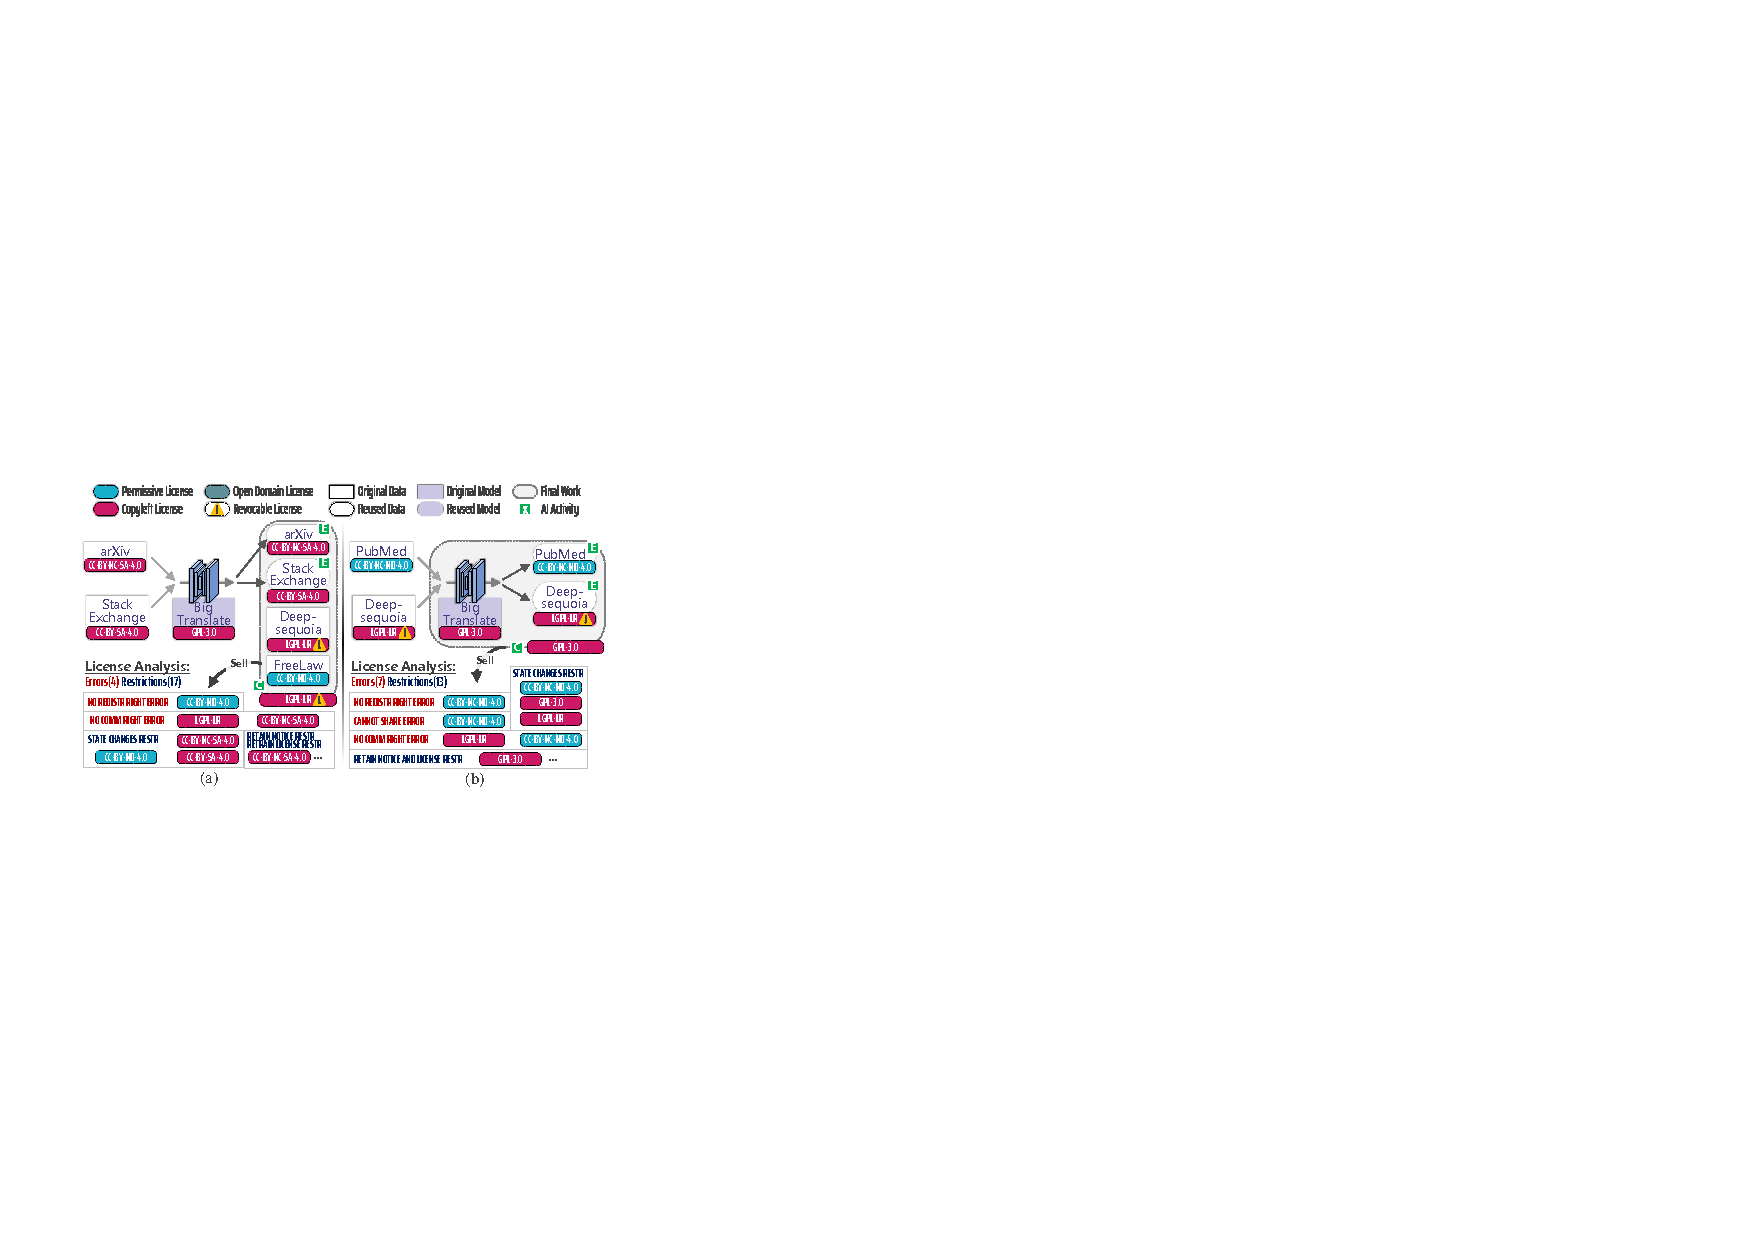
\includegraphics[width=\linewidth]{fig/case1.pdf}
    \caption{Case Study \Romannum{1}: Corpus Combination. (a) LGPL-LR proliferation, CC collection; (b) LGPL-LR no linguistic resource, CC No redistribution.}
    \Description{}
    \label{fig:case1}
\end{figure}

\begin{figure}[t]
    \centering
    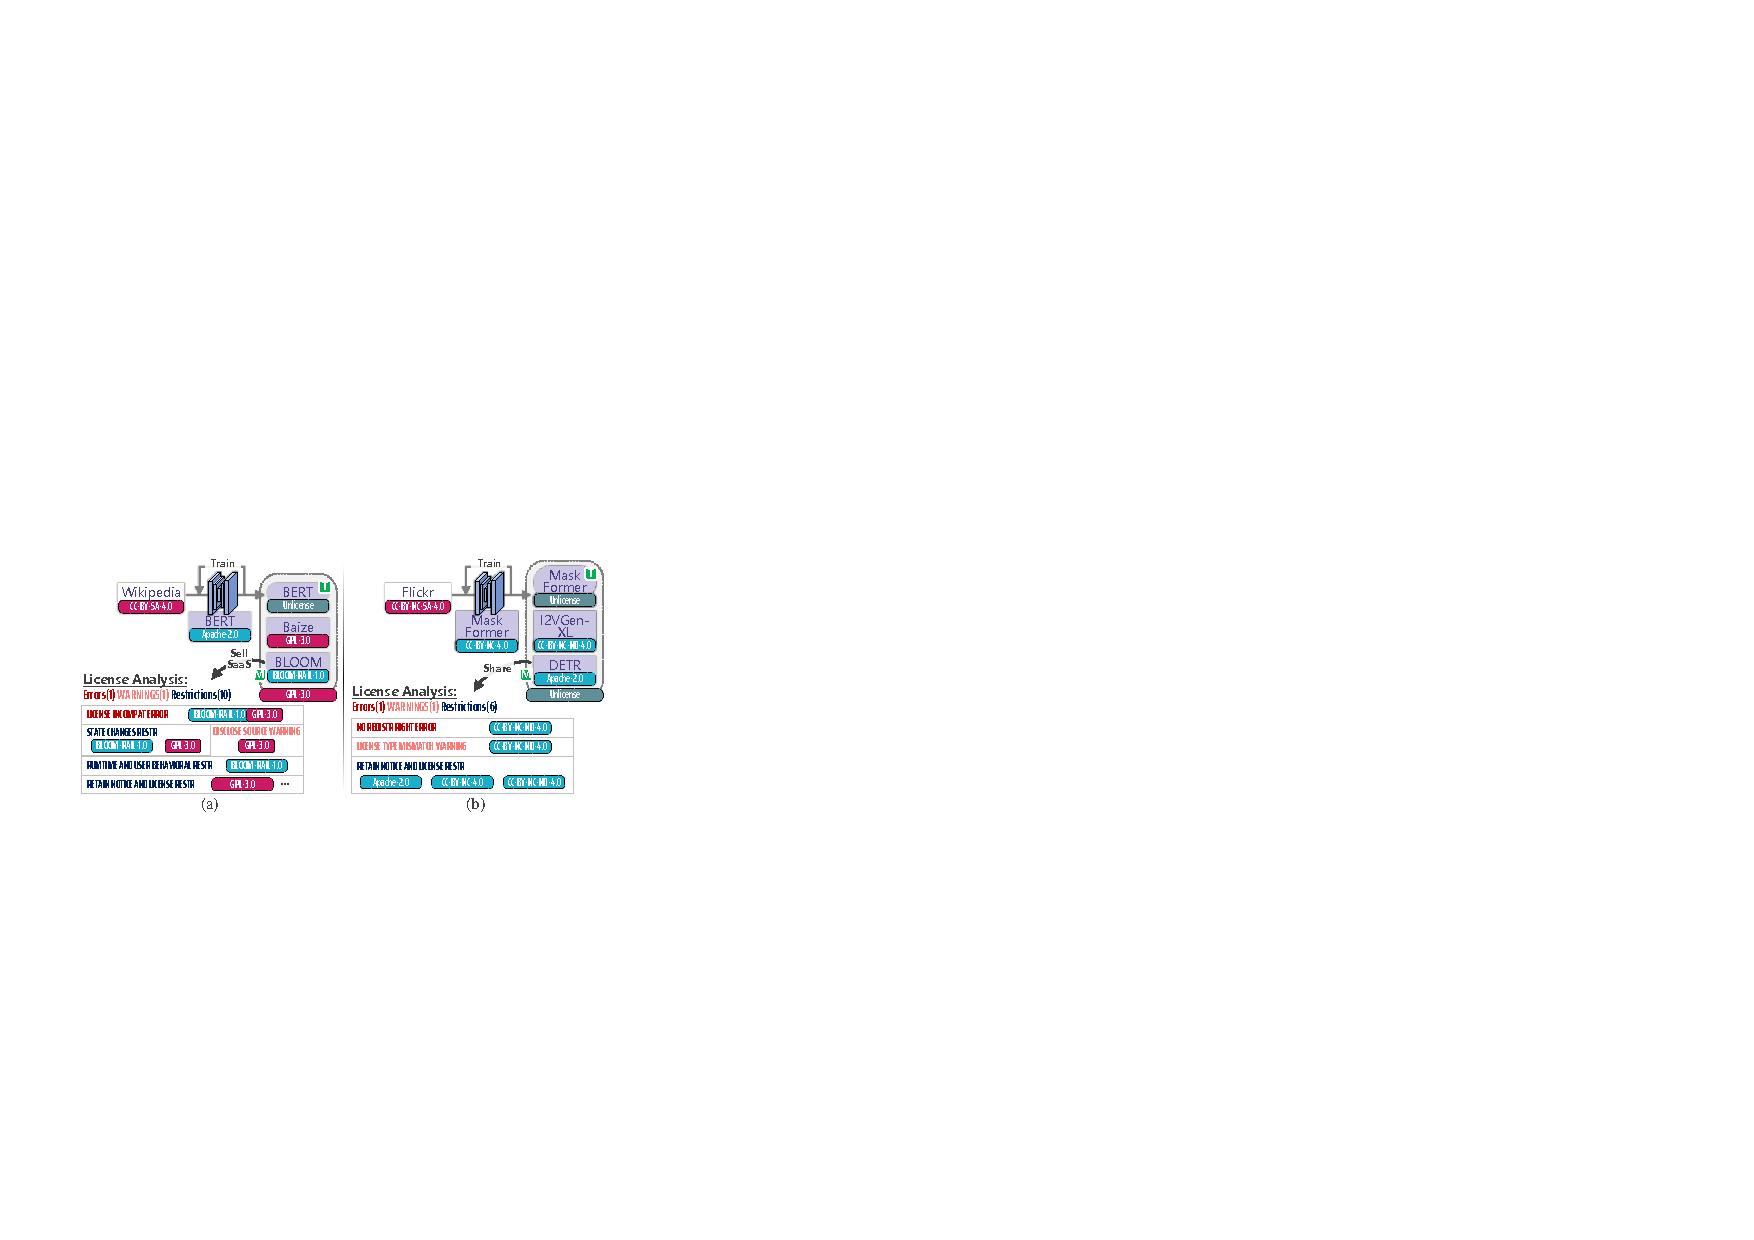
\includegraphics[width=\linewidth]{fig/case2.pdf}
    \caption{Case Study \Romannum{2}: Mixture of Experts. (a) BLOOM-RAIL, binary of GPL; (b) Unlicense, CC-BY-NC no distribute derivative. GPL Automatic Licensing of Downstream Recipients}
    \Description{}
    \label{fig:case2}
\end{figure}

\begin{figure}[t]
    \centering
    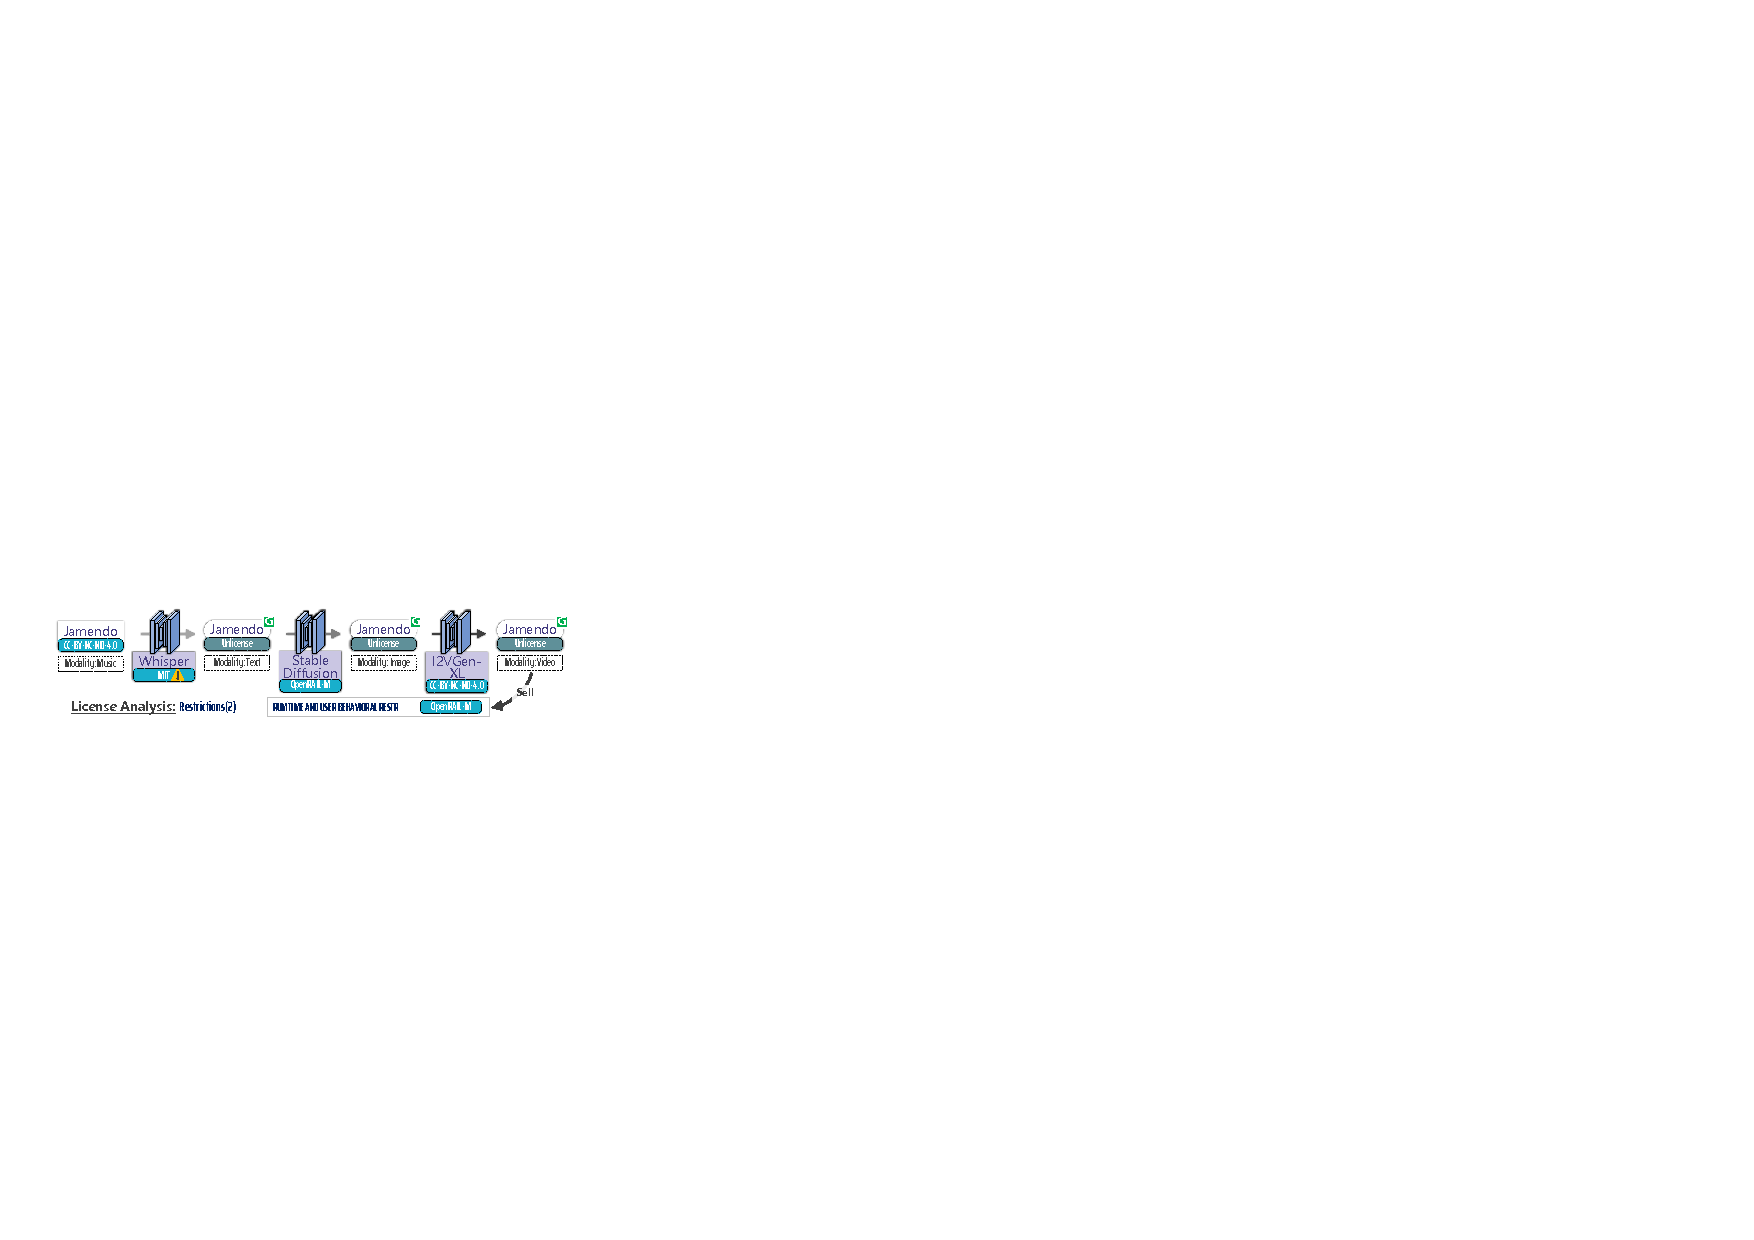
\includegraphics[width=\linewidth]{fig/case3.pdf}
    \caption{Case Study \Romannum{3}: Pipeline.}
    \Description{}
    \label{fig:case3}
\end{figure}

\begin{figure}[t]
    \centering
    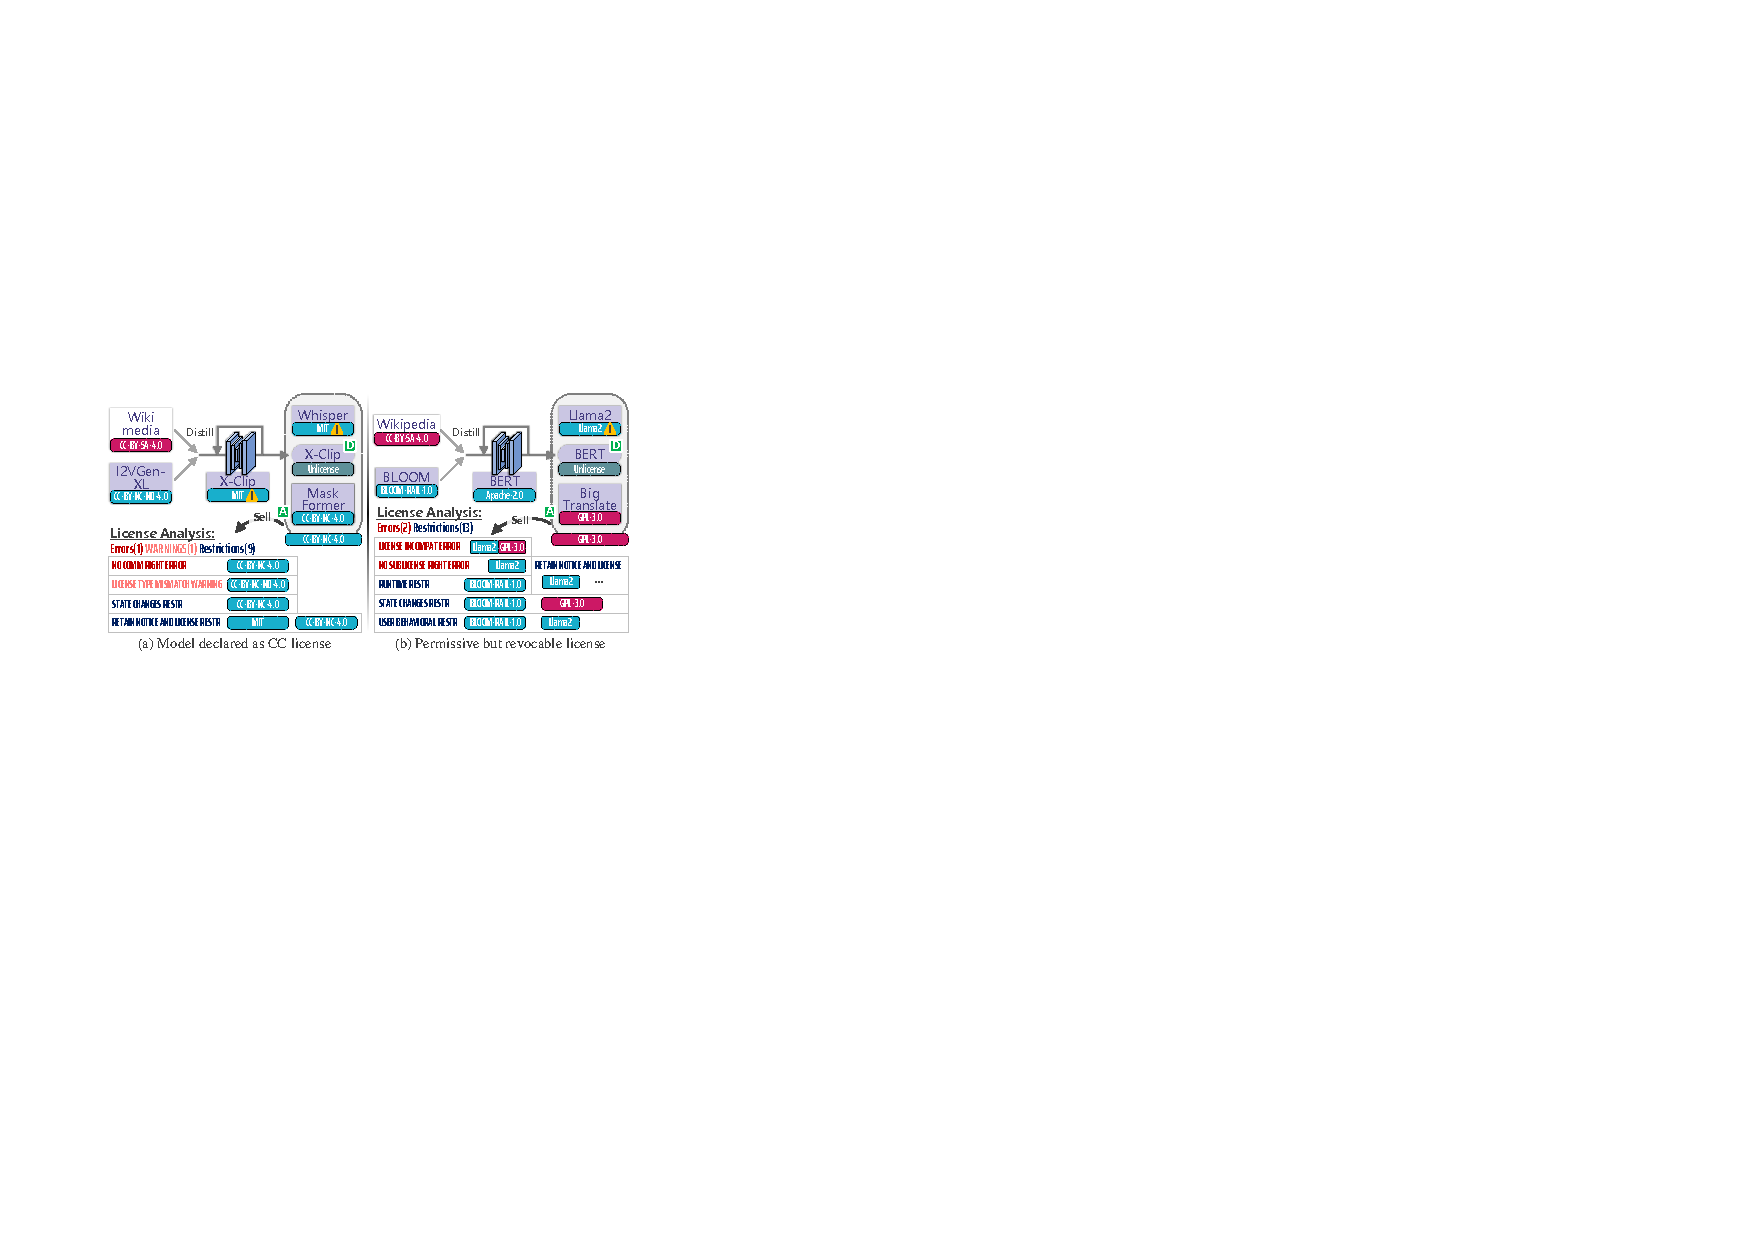
\includegraphics[width=\linewidth]{fig/case4.pdf}
    \caption{Case Study \Romannum{4}: distillation and model averaging.}
    \Description{}
    \label{fig:case4}
\end{figure}

\begin{figure}[t]
    \centering
    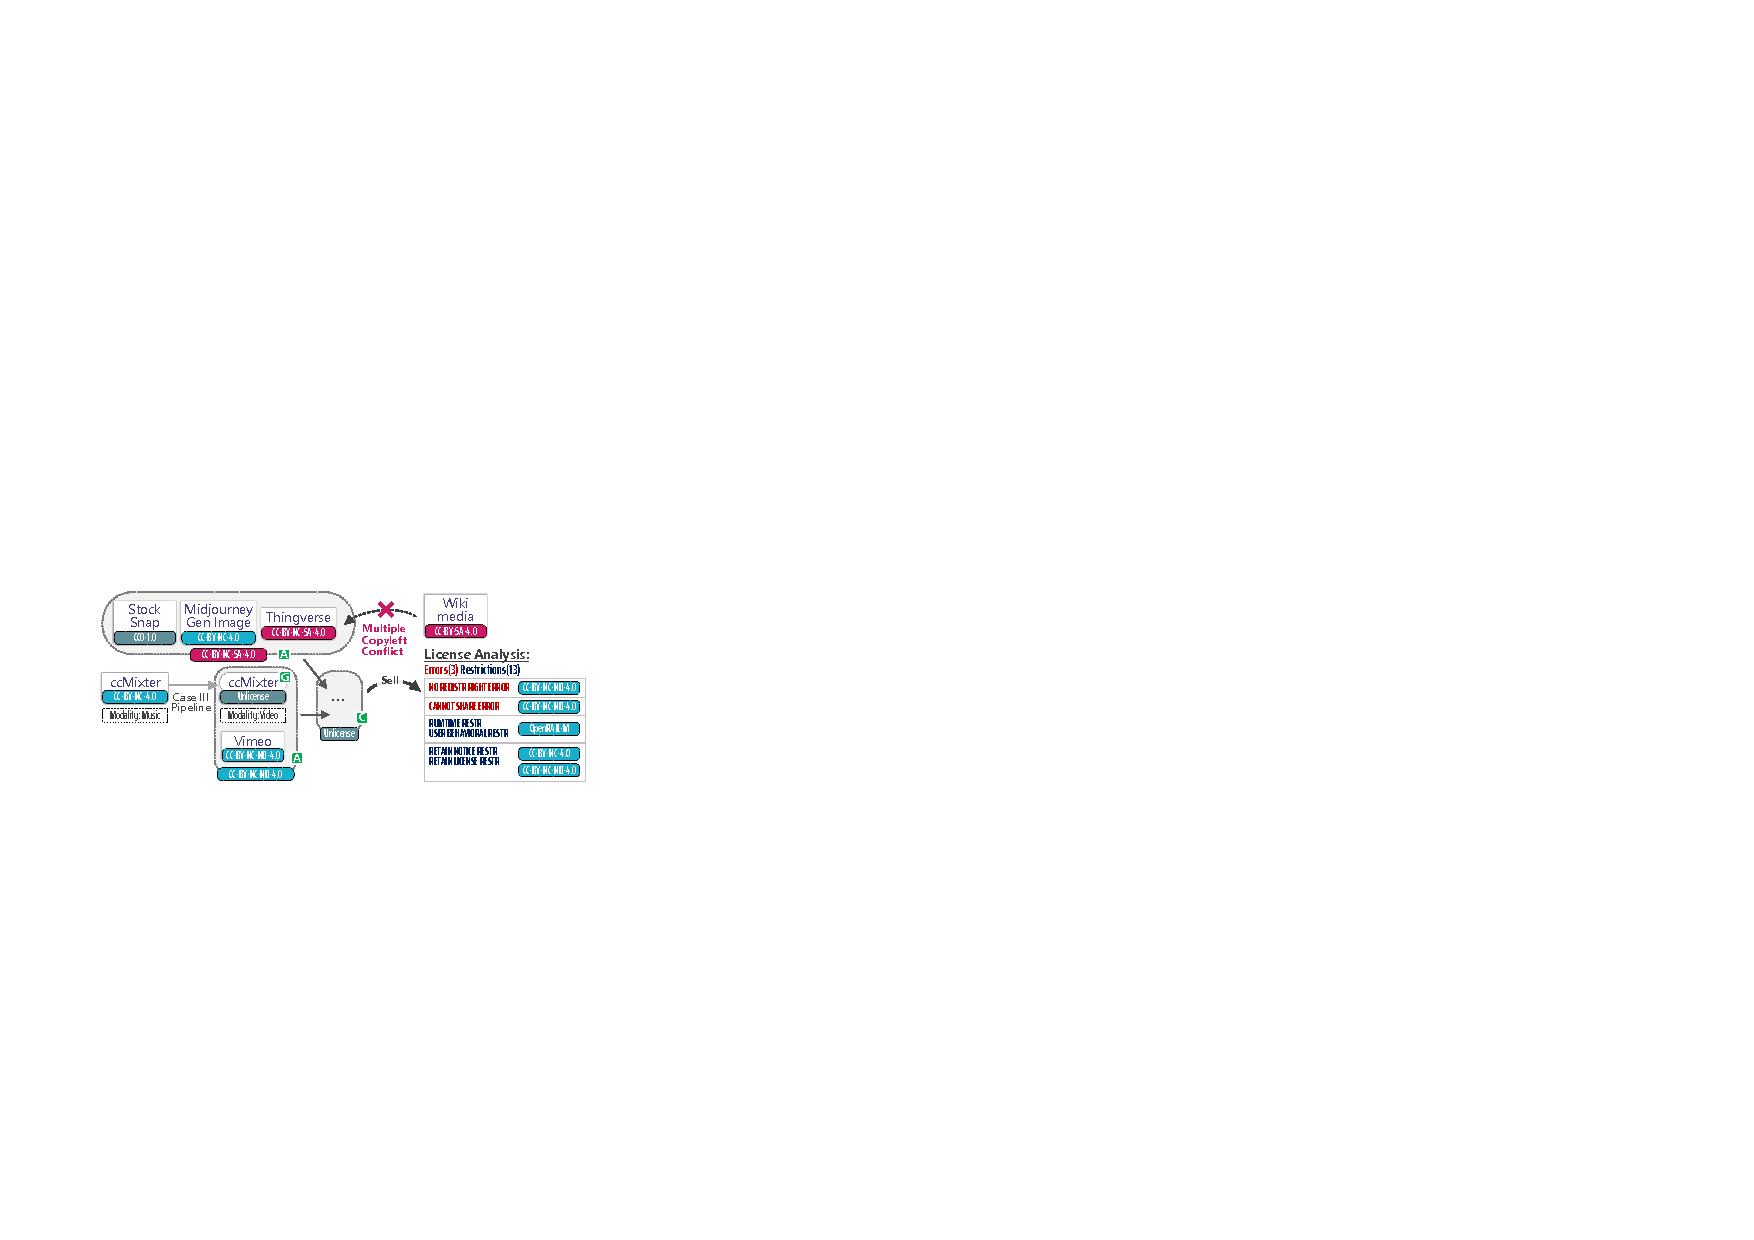
\includegraphics[width=\linewidth]{fig/case5.pdf}
    \caption{Case Study \Romannum{5}: distillation and model averaging.}
    \Description{}
    \label{fig:case5}
\end{figure}